\documentclass[a4paper,12pt,ngerman]{scrartcl}

% Language
\usepackage{polyglossia}
\setmainlanguage{german}

% Grafiken
\usepackage{graphicx}

% Make \today print in format "NN<st|nd|rd|th> MM YYYY"
\usepackage{isodate}
\origdate

\linespread{1.15}

% Titel anders formatieren mit: Command, Format, Label, Sep, Before-Code
\usepackage{titlesec}
\titleformat{\section}{\sffamily\Large\bfseries}{}{0pt}{}
\titleformat{\subsection}{\sffamily\large\bfseries}{}{0pt}{}

% Own pagestyle (header and footer)
\usepackage{fancyhdr}
\fancyhf{} % Clear header and footer content
\fancyhead[L]{{\small \textsf{WS 14/15, Informationsvisualisierung}}}
\fancyhead[C]{{\small \textsf{Übung 3}}}
\fancyhead[R]{{\small \textsf{\today}}}
\fancyfoot[C]{\thepage}

% Text in quotes
% Usage: \enquote{To be or not to be.}
\usepackage{csquotes}

% Subliminal refinements towards typographical perfection
\usepackage{microtype}

% Footnotes in section
\usepackage[stable]{footmisc}

% Better refs with \cref{}
\usepackage[capitalize,noabbrev]{cleveref}

% Borders
\usepackage[paper=a4paper,left=20mm,right=20mm,top=30mm,bottom=30mm]{geometry}

\usepackage{longtable}

\begin{document}
\pagestyle{fancy} % Activate own pagestyle

\section{Aufgabe 3.1 | Visuelle Eigenschaften von Graphen}
\subsection*{Layout}
Das Layout ist eines der zentralen Eigenschaften eines Graphen. Neben hierarchischen, kreisförmigen u.a. existiert das kraftbasierte Layout eines Graphen. Eine sinnvoller Einsatz ist folgender:

Als Eingabe verwendet man die GPS-Rohdaten vieler Personen die sich zwischen einigen Orten hin- und herbewegen (z.B. Kino, Zuhause, Einkaufszentrum). Eine Firma möchte nun zielgerichtet Werbung schalten und wissen wie die Leute sich zwischen diesen Orten bewegen. Da bei einem kraftbasierten Layout isomorphe Graphen sehr ähnlich dargestellt werden ist die visuelle Analyse der resultierenden Daten viel schneller als die anderer Layouts.

\subsection*{Visuelle Codierung}
Neben Form und Farbe ist die Größe eines Knotens ein Faktor beim visualisieren eines Graphen. Damit kann man z.B. in einem Freundesnetzwerk den Grad eines Knotens (Anzahl der Freunde) darstellen. Mehr Freunde $\rightarrow$ größerer Knoten und umgekehrt.

\subsection*{Rendering}
Mit Rendering ist die Änderung der Sichtweise auf den visualisierten Graphen gemeint. Interaktionen wie vergrößern und verkleinern sowie andere Interaktionsarten gehören zu dieser Eigenschaft eines Graphen. Sinnvolle Anwendungen ergeben sich in Domänen in denen zunächst eines Übersicht benötigt wird um anschließend einen detailierten Blick auf Teilgraphen (z.B. Cluster) zu werfen. Als Beispiel seien hier Warmwasserleitungen zwischen Städten (Übersicht) und innerhalb einzelner Städte (Detailansicht) zu nennen.

\subsection*{Vereinfachung}
Vereinfachungen oder Abstraktionen sind vom Vorteil wenn der zu visualisierende Datensatz zu groß ist um ihn komplett darzustellen. Dateisysteme sind komplexe Systeme und sind auf jedem erdenklichen System hierarchisch angeordnet. Diese hierarchische Anordnung stellt eine Form der Vereinfachung dar um sie für den Menschen greifbar erscheinen zu lassen. Anschließend kann man die verschiedenen Hierarchiestufen traversieren.

\section{Aufgabe 3.2 | Visual Clutter}
\subsection*{Kamada-Kawai}
\begin{itemize}
    \item Rahmenbedingungen
    \begin{itemize}
        \item ungerichtete, gewichtete Graphen
        \item gerade Kanten, keine Beschränkung bei Positionierung der Knoten
        \item zusammenhängender Graph (sonst: Zusammenhangskomponenten einzeln zeichnen)
    \end{itemize}
    \item Kriterien
    \begin{itemize}
        \item Anzahl Kantenkreuzungen reduzieren
        \item gleichmäßige Verteilung von Knoten und Kanten (wichtiger für menschliches Verständnis)
    \end{itemize}
    \item Idee
    \begin{itemize}
        \item Stahlringe werden durch Federn zusammengehalten
        \item Ziel: Minimierung der Energie dieses Systems
        \item ideale Distanz zwischen zwei Knoten proportional zur Länge eines kürzesten Pfades zwischen ihnen
    \end{itemize}
    \item Algorithmus
    \begin{itemize}
        \item Berechnung der Distanz $d_{i,j}$  (Shortest Path Algorithm - Floyd), in gewichteten Graphen: Distanz = Summe der Gewichte
        \item Berechnung der Länge $l_{i,j}$ (aus Distanz und optimaler Länge)
        \item Berechnung der Federstärke $k_{i,j}$ (aus Distanz)
        \item Bestimmung der initialen Knotenpositionen
        \item Schrittweise Minimierung der Energie: Verschieben eines Knotens in stabile Position
    \end{itemize}

    Laufzeit: O($|V|^3 + T * |V|$), $T =$ Anzahl der Iterationen

    \item Besonderheiten
    \begin{itemize}
        \item symmetrische Graphen werden auch symmetrisch angeordnet
        \item isomorphe Graphen werden auf dieselbe Art und Weise dargestellt (evtl. verschoben, gedreht oder gespiegelt)
    \end{itemize}
\end{itemize}


\subsection*{Fruchtermann-Reingold}
\begin{itemize}
    \item Rahmenbedingungen
    \begin{itemize}
        \item ungerichtete Graphen
        \item gerade Kanten, Graph begrenzt durch festen Rahmen
    \end{itemize}
    \item Kriterien
    \begin{itemize}
        \item gleichmäßige Verteilung von Knoten und Kanten innerhalb des Rahmens
        \item Anzahl Kantenkreuzungen reduzieren
        \item Streben nach symmetrischer Darstellung
        \item Nachbarknoten sollen nah beieinander liegen, Knoten sollen aber nicht zu eng zusammen gezeichnet werden
    \end{itemize}
    \item Idee
    \begin{itemize}
        \item Knoten verhalten sich wie Atomteilchen und üben anziehende und abstoßende Kräfte aufeinander aus
        \item zur Vereinfachung: anziehende Kräfte nur zwischen Nachbarknoten, abstoßende Kräfte zwischen allen Knoten
        \item Geschwindigkeit statt Beschleunigung, statisches Gleichgewicht statt dynamischem Gleichgewicht
    \end{itemize}
    \item Algorithmus
    \begin{itemize}
        \item Berechnung der abstoßenden Kräfte
        \item Berechnung der anziehenden Kräfte
        \item Verschiebung begrenzen durch Temperatur
        \item Teilchen am Rahmen stoppen
        \item Sonderfall: zwei Knoten mit derselben Position $\rightarrow$ behandeln als wären sie dicht beieinander, dann wirken große abstoßende Kräfte
    \end{itemize}

    Laufzeit: O(T * ($|V|^2 + |E| + |V||E|$)), $T =$ Anzahl der Iterationen $=$ O(|V|) oder O(|E|)

    \item Variante des Algorithmus
    \begin{itemize}
        \item Einteilung in Gitter
        \item abstoßende Kräfte nur zwischen Knoten benachbarter Quadrate
        \item besser: abstoßende Kräfte zwischen Knoten innerhalb eines Kreises um Ausgangsknoten
    \end{itemize}

    Laufzeit: O(T * ($|V| + |E| + |V||E|$)), $T =$ Anzahl der Iterationen $=$ O(|V|) oder O(|E|)
    \item Ergebnisse
    \begin{itemize}
        \item symmetrische Graphen werden besonders gut dargestellt
        \item nicht alle symmetrischen, planaren Graphen werden optimal dargestellt
        \item isomorphe Graphen werden auf dieselbe Art und Weise dargestellt (evtl. verschoben, gedreht oder gespiegelt)
        \item relativ viele Kantenkreuzungen bei Bäumen, Wurzel nicht zu erkennen
        \item sehr unterschiedlich gute Ergebnisse bei dreidimensional wirkenden Graphen
        \item Variante: Dreidimensionales Layout
    \begin{itemize}
        \item Layouting in drei Dimensionen, Projektion in die Ebene
        \item keine Verbesserung der Ergebnisse im Vergleich zum 2D-Algorithmus
        \item Auswahl der Projektion durch Benutzer
    \end{itemize}
    \item Zusammenhangskomponenten driften auseinander und verbreiten sich am Rand $\rightarrow$ einzelne Berechnungen (wie bei Kamada-Kawai) oder Gitter-Variante
    \item sehr schnelle Berechnungen
    \end{itemize}
\end{itemize}

\subsection*{Gemeinsamkeiten \& Unterschiede}
\begin{itemize}
    \item Layouting ungerichteter Graphen mit geraden Kanten, Kamada-Kawai unterstützt auch gewichtete Graphen, Fruchtermann-Reingold ordnet Graphen innerhalb eines festen Rahmens an
    \item Ziel beider Verfahren: gleichmäßige Verteilung der Knoten und Kanten, Kamada-Kawai dabei eher fixiert auf Vermeidung von Kantenkreuzungen
    \item verschiedene Ideen liegen zugrunde: System aus Federn $\leftrightarrow$ Kräfte zwischen Atomteilchen
    \item verschiedene Laufzeiten, Fruchtermann-Reingold wesentlich schneller
    \item gute Darstellungen symmetrischer und isomorpher Graphen, Fruchtermann-Reingold Probleme mit komplexeren Graphen
\end{itemize}

\section{Aufgabe 3.3 | Graphen übersichtlicher gestalten}

\subsection*{Gruppieren von Knoten und Kanten}
Besteht ein Graph aus besonders vielen Knoten und Kanten, können diese eventuell zu Gruppen zusammengefasst werden. Ob dies das Verständnis erleichtert, ist jedoch immer abhängig vom Inhalt bzw. der Bedeutung der Daten. Beispielsweise könnten in einem Netzwerk, das über die gesamte Welt verteilt ist, Einheiten nach Ländern gruppiert  und somit die Beziehungen zwischen den Ländern dargestellt werden.

\subsection*{Einfärben von Knoten oder Kanten}
Eine weitere Möglichkeit, einen Graphen übersichtlicher zu gestalten, ist ihn mit Farbe zu versehen. Können die Knoten oder Kanten thematisch gruppiert werden, erleichtert es das Verständnis, wenn diese Gruppen durch unterschiedliche Farben repräsentiert werden. So kann sich schneller ein Überblick verschafft werden. Zudem erleichtert es das Erkennen interner sowie externer Beziehungen dieser Gruppen.

\subsection*{Verschiedene Knotendarstellungen}
Lassen sich die Knoten in Gruppen einteilen und ist der Graph nicht allzu groß, könnten verschiedene Knotendarstellungen eingesetzt werden, um die Zugehörigkeit zu einer Gruppe darzustellen. Dies könnten z.B. einfache Formen wie Kreise, Quadrate, Sterne etc. sein, oder aber auch spezifische Darstellungen, die eine direkte Repräsentation der Gruppen ermöglicht.

\subsection*{Interaktionstechniken}
Mittels Interaktion lassen sich Graphen übersichtlicher gestalten. Zoomen, verschieben oder das visuelle Hervorheben spezieller Zusammenhänge durch anklicken etc. vermindern eine zu hohe kognitive Belastung und tragen so zur Übersichtlichkeit gerade sehr komplexer Graphen dar. Auch durch das spielerische Wesen der Interaktion können so komplexe Sachverhalte mit reduzierter Schwierigkeit betrachtet und analysiert werden.

\section{Aufgabe 3.4 | Visualisierung mit Gephi}

%\begin{figure}[ht]
%    \centering
%    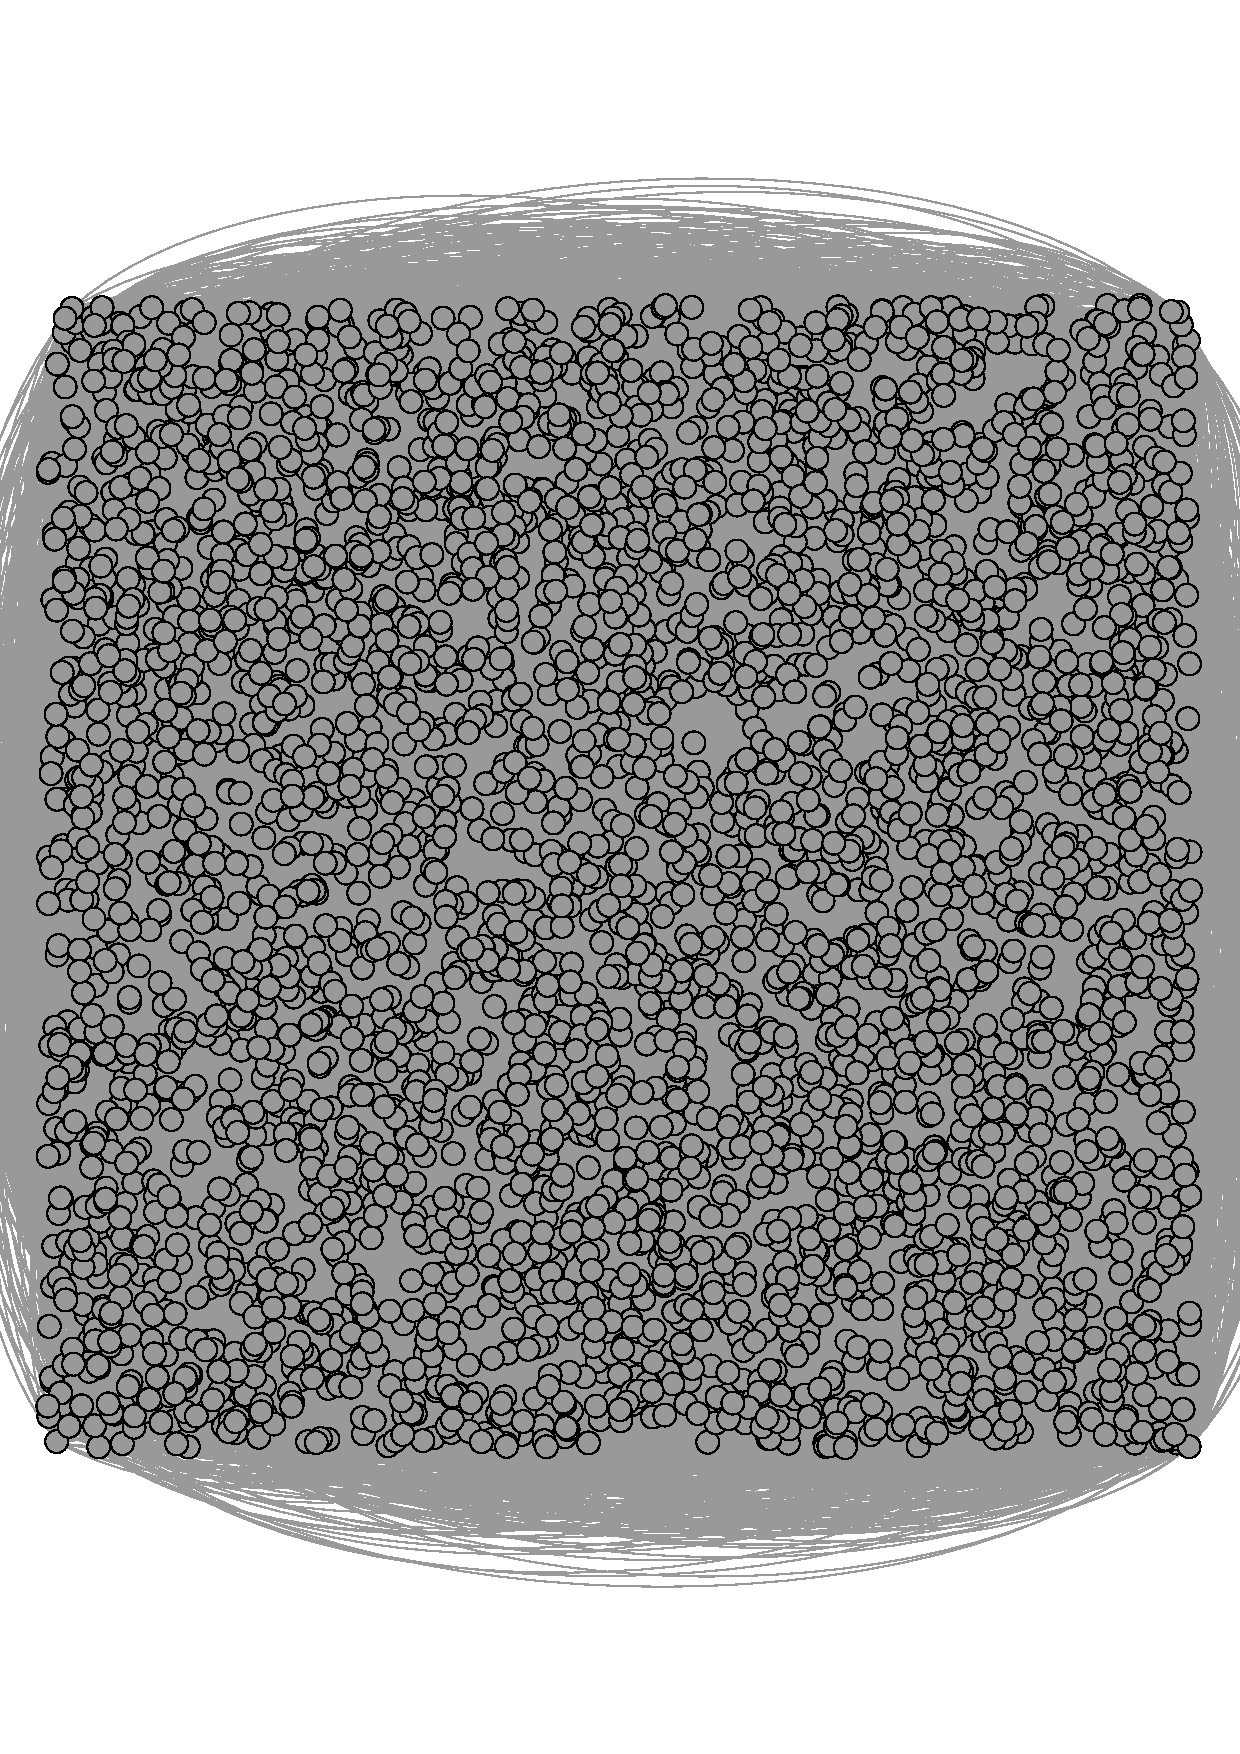
\includegraphics[height=8cm]{includes/gephi1}
%    \caption{Grafik direkt nach Import der Daten}
%    \label{fig:gephi1}
%\end{figure}
%
%\begin{figure}[ht]
%    \centering
%    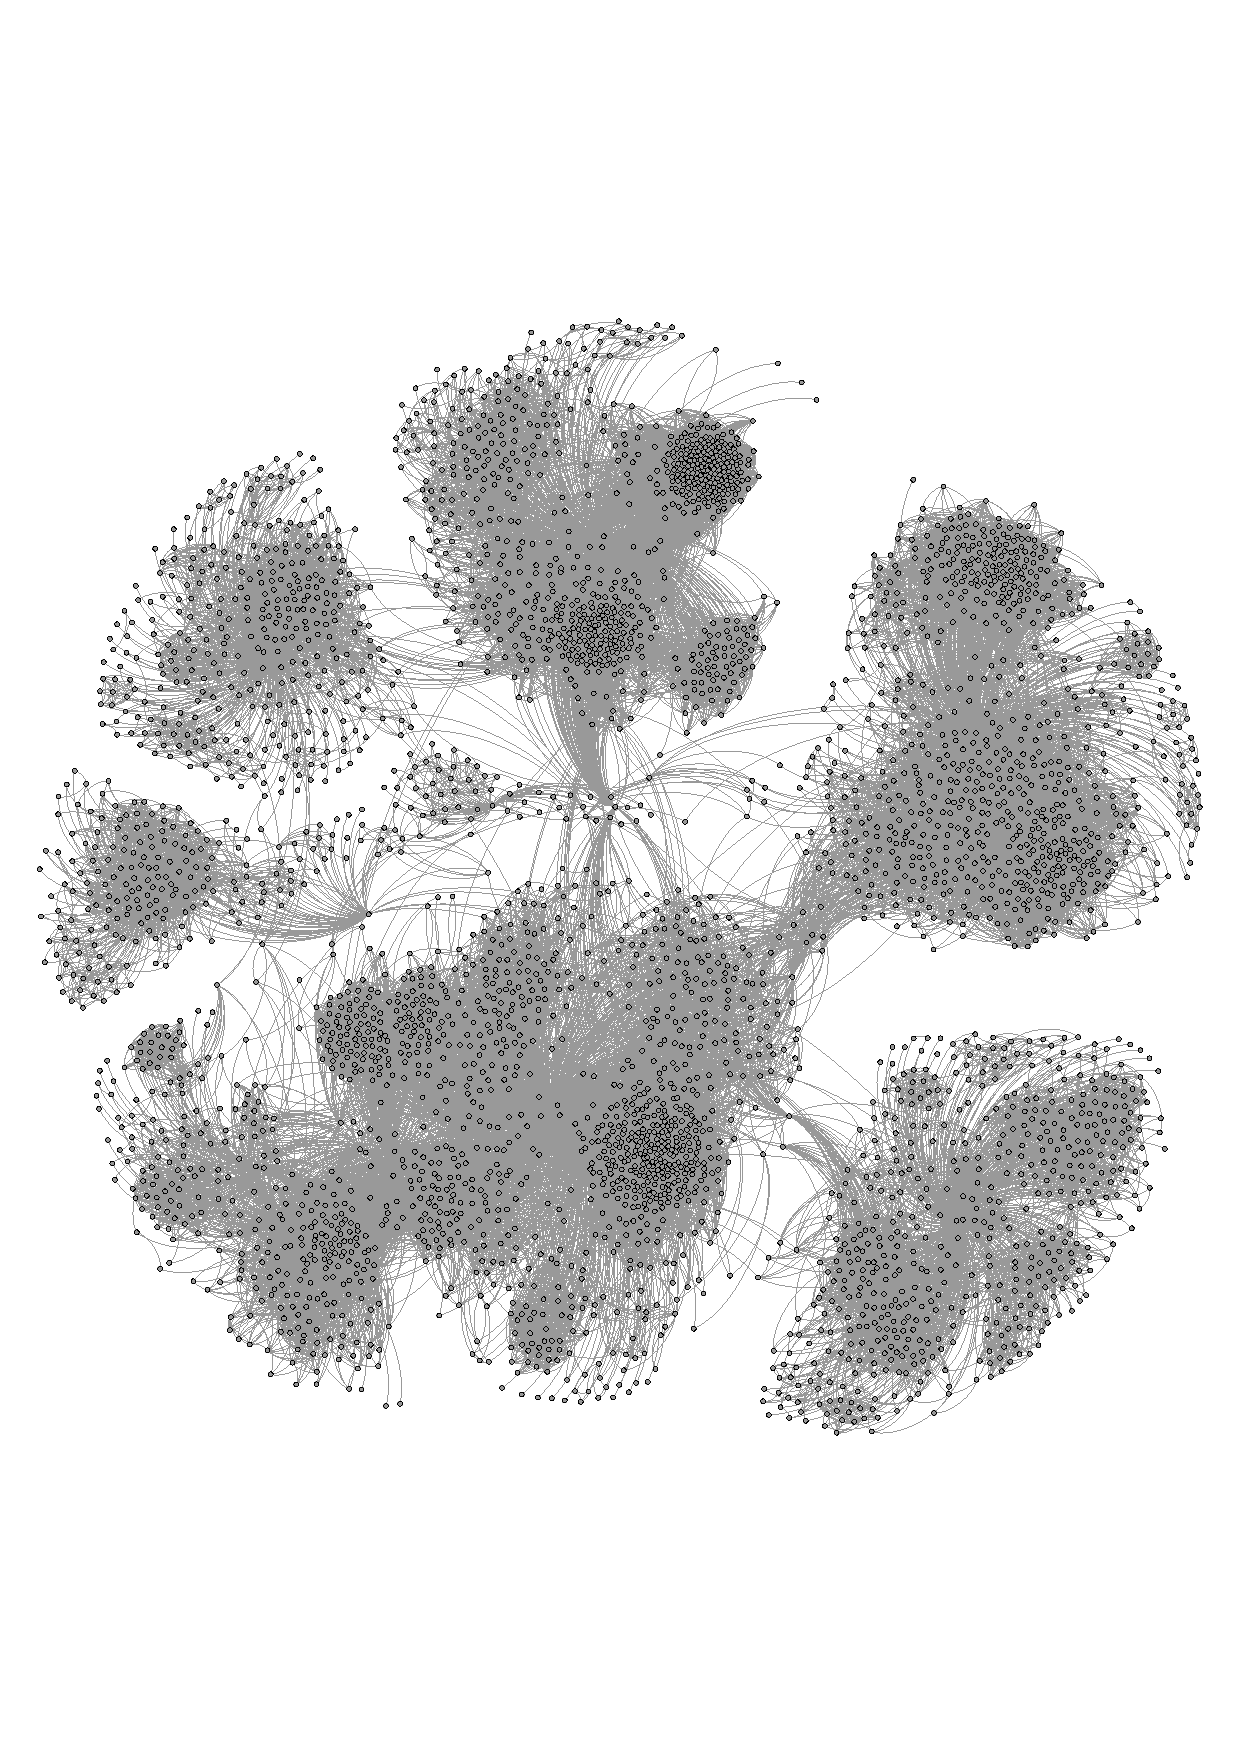
\includegraphics[height=8cm]{includes/gephi2}
%    \caption{Grafik direkt nach Import der Daten}
%    \label{fig:gephi2}
%\end{figure}

Für die Visualisierungen mit Gephi wird hier der Datensatz der Facebook-Freundschaften der empfohlenen Seite verwendet, der aus 10 Netzwerken zusammengesetzt wurde \footnote{Größere Datensätze waren im CIP-Pool leider nicht zu importieren. Selbst mit diesem relativ kleinen Datensatz gab es immer wieder Probleme mit dem begrenzten Speicherplatz. Auf meinem Windows-PC wollte Gephi leider nicht starten.}.

Gephi beginnt nach dem Import des Datensatzes mit einem zufälligen Layout, das die Knoten innerhalb einer rechteckigen Fläche anordnet, siehe \cref{fig:start}. In dieser Darstellung sind bei Datensätzen solcher Größe vermutlich selten Aussagen über die Daten zu treffen.

\begin{figure}[ht]
    \centering
    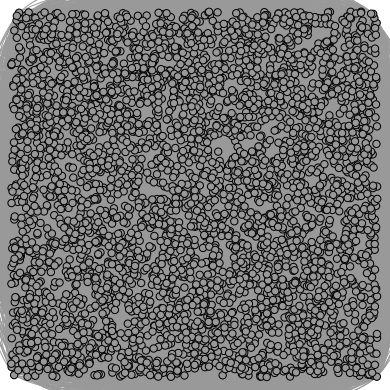
\includegraphics[height=8cm]{includes/snapshot_start}
    \caption{Grafik direkt nach Import der Daten}
    \label{fig:start}
\end{figure}

In erster Linie kann die Visualisierung durch ein Layout verbessert werden, das nach den Beziehungen zwischen den Daten ausgerichtet ist. Die Erfahrung zeigt, dass oft eine Kombination verschiedener Algorithmen ästhetischere Abbildungen ergibt, aus denen bereits erste Erkenntnisse gewonnen werden können. \Cref{fig:einfarbig} zeigt ein solches Layout.

\begin{figure}[ht]
    \centering
    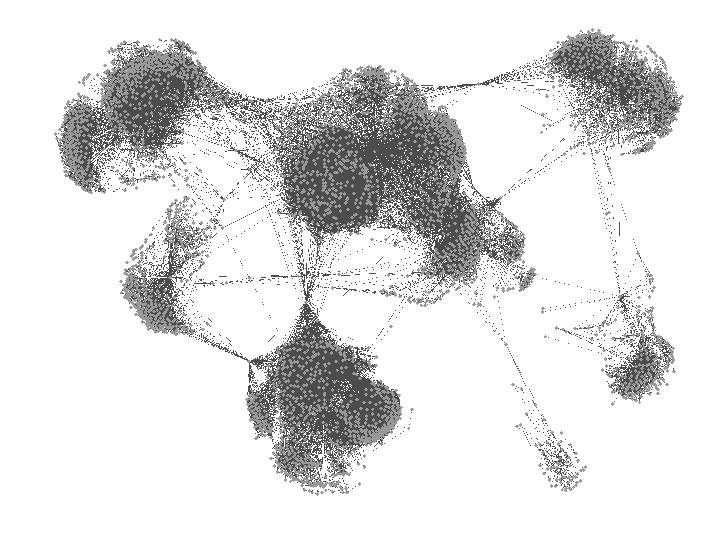
\includegraphics[height=8cm]{includes/snapshot_einfarbig}
    \caption{Grafik nach Anwendung von Layout-Algorithmen}
    \label{fig:einfarbig}
\end{figure}

Zusätzlich können Knoten und Kanten noch eingefärbt werden. Zu den zahlreichen Möglichkeiten gehören unter anderem (Ein-/Ausgangs-)Grad, Kantengewicht oder Zentralitätsmaße. Am nützlichsten hat sich für diesen Datensatz die Färbung der Knoten nach \emph{Modularity} erwiesen, wie in \cref{fig:bunt} zu sehen.

\begin{figure}[ht]
    \centering
    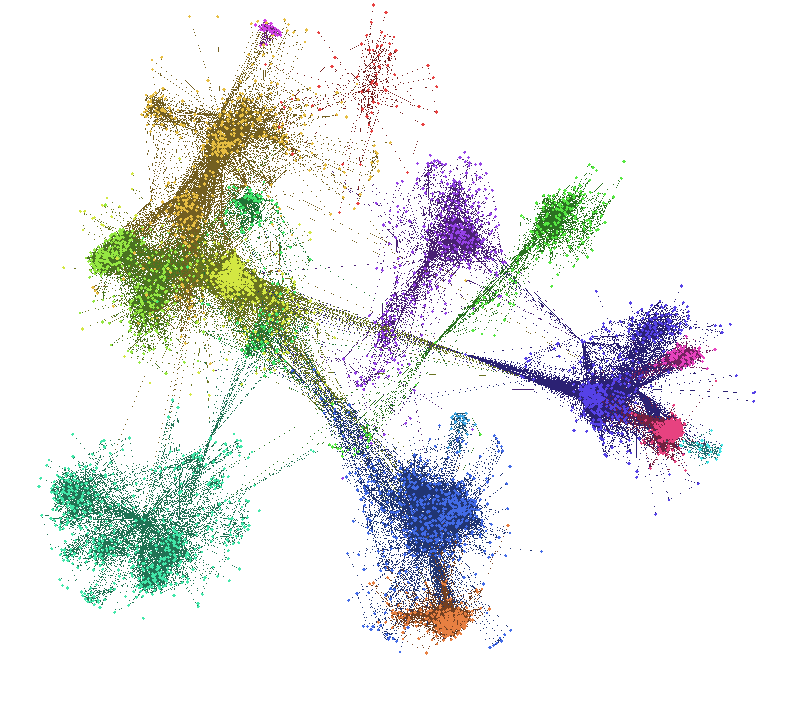
\includegraphics[height=8cm]{includes/snapshot_bunt}
    \caption{Grafik nach Anwendung von Layout-Algorithmen und Einfärben der Knoten}
    \label{fig:bunt}
\end{figure}

\end{document}
